\documentclass[11pt]{article}

\usepackage{report}

\usepackage[utf8]{inputenc}
\usepackage[T1]{fontenc}
\usepackage[colorlinks=true, linkcolor=black, citecolor=blue, urlcolor=blue]{hyperref}
\usepackage{url}
\usepackage{booktabs}
\usepackage{amsfonts}
\usepackage{amsmath}
\usepackage{nicefrac}
\usepackage{microtype}
\usepackage{graphicx}
\usepackage{natbib}
\usepackage{doi}
\usepackage{minted}
\usepackage{subfig}
\usepackage{titlesec}
\setcitestyle{aysep={,}}

\titleformat{\subsubsection}
  {\selectfont}{\thesubsubsection}{1em}{}


\title{Predicting Food Groups \\ \vspace{0.5em} \large from nutritional information}

\author{
    David Sha\\
\AND
    Victoria Lyngaae\\
\AND
    Mason Sebek\\
\AND
    William Spongberg\\
\AND
\AND
	COMP20008: Elements of Data Processing\\
\AND
	The University of Melbourne\\
}

\date{May 2023}

\renewcommand{\headeright}{Predicting Food Groups from Nutritional Information}
\renewcommand{\undertitle}{Report}
\renewcommand{\shorttitle}{}

\begin{document}
\maketitle

\newpage
\tableofcontents
\thispagestyle{empty}

\newpage
\setcounter{page}{1}
\section{Introduction}

In this report, we will be analysing a food dataset from \cite{FoodStandardsAustraliaNewZealand}. Using the $k$-nearest neighbours algorithm, we build a model that predicts the food groups of a particular food item based on its nutritional information and explore how useful this model is to the food industry.

% The objective of this project is to wrangle and analyse data contained within the \cite{FoodStandardsAustraliaNewZealand} dataset, for the purpose of answering an explicit and defined research question. We propose the inquiry: Can we predict the food group of a food item, based solely on its nutritional information? We implemented the supervised learning model of $k$-nearest neighbours to predict and explore the relationship between nutritional information and food group classification.

\subsection{Research Question}
% 1. What is the research question?
To what extent can we predict the food group of a food item based solely on its nutritional information?

\subsection{Target Audience}
% 2. Who are the target audience.
The outcome of this report may be interesting to major supermarket chains such as Coles or Woolworths. If the model is sufficiently accurate, it could be useful in detecting food items that may or may not be labelled correctly or are missing labels in a particular batch of food items sent to a store. Better classification of food items would improve a supermarket's inventory management as well as its product placement, which will ultimately improve the shopping experience of customers.

% The findings of this exploration may be of value to a number of audiences, such as nutritionists, health researchers, consumers, educational institutions and food retailers.  An effective food group classification model has many practical applications such as:
% \begin{itemize}
%     \item Detection of food items that are labelled incorrectly, either by accident or with the intent to mislead consumers
%     \item Improving a retailer's inventory management and product placement, and ultimately a customer's shopping experience
%     \item Effective assessment of an individual's nutritional intake and dietary pattern
%     \item Educating and enhancing public understanding of food groups, and general nutritional literacy
% \end{itemize}



\subsection{Dataset}
% 3. The dataset you have chosen.
We make use of the dataset from \cite{FoodStandardsAustraliaNewZealand} containing 1616 food items and their nutritional information. This dataset contains all the information we need to answer our research question as each food item has a \verb|Classification| (food group) and respective nutritional information (such as energy, protein, etc.). We also use a complementary dataset from \cite{FoodClassification} which maps numerical classifications to their respective food groups which becomes very useful when providing some domain context during preprocessing and analysis.

\section{Methodology}

\emph{What wrangling and analysis methods (including at least one supervised learning method) have you applied? Why have you chosen these methods over other alternatives? How do you perform the experiment?}

During the initial stages of our investigation, we debated over linear regression on a continuous variable such as \verb|Energy with dietary fibre, equated (kJ)| or $k$-nearest neighbours on a categorical variable such as \verb|Classification|. We explored both options and found it more interesting and more valuable to tackle the latter. All data wrangling techniques are implemented in \verb|preprocessing.ipynb| and all supervised learning and analysis techniques are implemented in \verb|knn.ipynb|.
% During the first stages of our investigation, we explored different target variables given any subset of the nutritional information. We initially considered predicting the \verb|Classification| of a food item but found that the number of unique classifications was too large to be useful. Then we pivoted for some time toward predicting the \verb|Energy|

\subsection{Data Wrangling}

\subsubsection{Preprocessing}

Prior to any use of machine learning, we evaluated  the quality of the data and found that it was not clean. Thus, we implemented various preprocessing techniques to ensure that the data was suitable to be included in the data pipeline. 


A large number of food items were wholly missing particular nutrition values. Understanding that this is likely an indication that a food has either an absence of the nutrient (eg, 0g) or that the food has not been checked for the nutrient's presence, we chose to set all NaN values to 0. Next, given that Food Standards Australia New Zealand (2013) indicates that the first two digits of a food's \verb|Classification| denote its major food group, each item's classification was simplified to these two characters. Doing so reduced the number of unique classifications drastically (from 290 to 23), which made our $k$-nn supervised learning model more effective later on. Given that there are now 23 unique food groups, as seen in Figure \ref{fig:food-group-distribution}, we also chose to simplify and compress less populated food groups, i.e., those containing very few food items, into a broader group, named \verb|Miscellaneous|.

\begin{figure}[htbp]
    \centering
    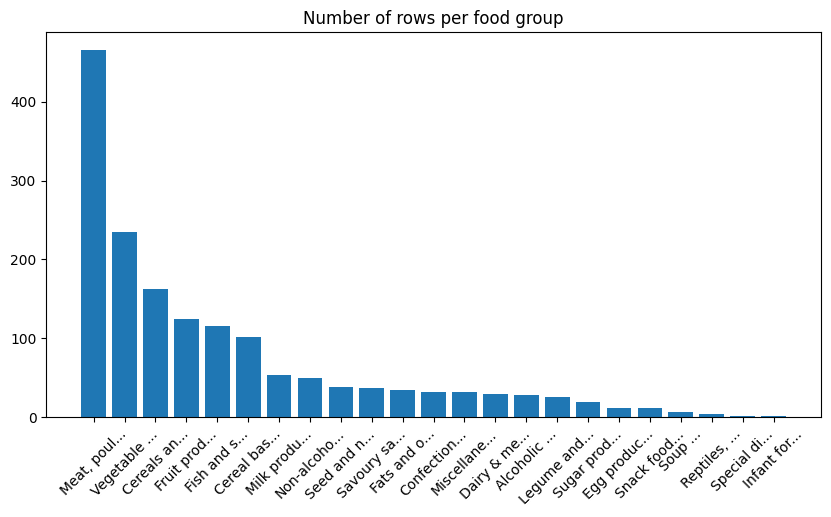
\includegraphics[width=0.9\textwidth]{report/figs/number-of-rows-per-food-group.png}
    \caption{The distribution of food items in twenty-three unique food groups not including unclassified items in the \cite{FoodStandardsAustraliaNewZealand} dataset.}
    \label{fig:food-group-distribution}
\end{figure}

However, rather than arbitrarily choosing a number of food groups to be condensed into \verb|Miscellaneous| (group 31), we opted to explore 3 different versions of the miscellaneous grouping; with 23, 14, and 6 groups (including the miscellaneous group) respectively condensed into \verb|Miscellaneous|. This can also be understood as providing the machine learning model with 6, 14 and 23 total labels, respectively for each variation.

\subsubsection{Feature Selection}

We also utilised \verb|mutual_info_classif| from \verb|sklearn|'s feature selection Python module to evaluate which nutritional features contained the most useful information for classification. With each food item having up to 290 different nutritional measures, the data is highly dimensional, and thus, through feature selection, we can improve the effectiveness of the $k$-nn model. With the mutual information calculated, by choosing an appropriate threshold (\verb|THRESHOLD=0.2| in \verb|preprocessing.ipynb|), we could remove some features that were not particularly insightful. This was done for each set of food groups, to ensure that they could be compared fairly.

We had initially considered using linear regression, but opted to continue our investigation using $k$-nn, as our research question required that our target variable be categorical/discrete, rather than continuous.  This is why, in \verb|preprocessing.ipynb|, we show working for both \verb|./archive/linear-regression.ipynb| and \verb|./src/knn.ipynb|, but only include the latter in the \verb|src| directory.

\subsection{Supervised Learning}

\subsubsection{Training and Test Split}

With our data preprocessed and cleaned, we decided to use an 85\% to 15\% train/test split (\verb|TEST_SPLIT=0.15| in \verb|knn.py|). The model was created using only the \verb|train| data, to ensure that the model could be fairly tested and evaluated based on its performance on unseen data, thus avoiding overfitting and ensuring generalisation.

% TODO: where to know the percentages?
We also employed a 10-fold cross validation approach to optimise the value of $k$ for each set of food groups. Calculating the mean accuracy of the cross validated $k$-nn model for a wide range of $k$ values (Figure \ref{fig:knn-cross-validation}) revealed that a $k$ of 1 performed best for each variation. Given that a $k$ value of 1 may potentially cause the model to be overfitted, as stated from \cite{StackExchangePost}, it was decided to err on the side of caution and opt for each variation's next best $k$, especially given this is not wholly detrimental to the model's accuracy. This procedure can be seen in detail in \verb|knn.py| under the $k$-nn heading in the first function \verb|cross_validate()|.

\begin{figure}[htbp]
    \centering
    \subfloat[\centering 6 food groups]{{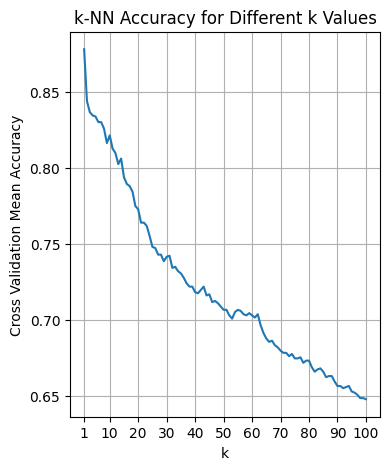
\includegraphics[height=5cm]{report/figs/knn-cross-validation-first.png} }}
    \qquad
    \subfloat[\centering 14 food groups]{{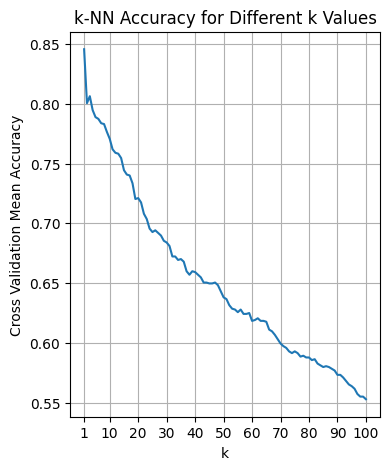
\includegraphics[height=5cm]{report/figs/knn-cross-validation-second.png} }}
    \qquad
    \subfloat[\centering 23 food groups]{{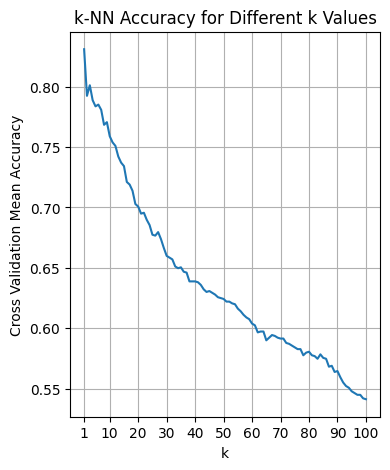
\includegraphics[height=5cm]{report/figs/knn-cross-validation-third.png} }}
    \caption{The $k$-nn cross validation mean accuracy for the 6, 14 and 23 food group classification models.}
    \label{fig:knn-cross-validation}
\end{figure}

Continuing with each variation's optimal, we also evaluated the final $k$-nn models using cross validation. By splitting the test data into 7 folds, (to somewhat emulate the 85\% to 15\% training and test split), we were able to evaluate whether our model could consistently and accurately predict a food item's food group, even when trained and tested on different sections of the preprocessed data; i.e., verify that the initial success of the model was not a fluke.

The data was also evaluated using bootstrap validation, where the $k$-nn model's performance was measured against random subsets of the original data. Bootstrap samples were created using randomly selected data points and the $k$-nn model trained upon them 1000 times, the high number of samples allowing for more accurate performance metrics. This validation reduces bias introduced by $k$-nn from the single training-test split and enhances the model's accuracy assessment by ensuring a more robust and unique evaluation every time it is run.

\section{Results}
\emph{What are the key results your research has obtained?}

\SaveVerb{knn}|knn.ipynb|
\SaveVerb{evaluation}|Evaluation|
\begin{table}[h]
    \centering
    \begin{tabular}{|l|c|c|c|c|}
        \toprule
        & $k$ & Accuracy & CV Mean Accuracy & Bootstrap Mean Accuracy \\
        \hline
        Top 6     & 2 & 88.48\% & 84.78\% & 90.83\% \\
        Top 14    & 3 & 85.19\% & 81.31\% & 86.58\% \\
        Top 23    & 3 & 83.95\% & 80.69\% & 85.80\% \\
        \bottomrule
    \end{tabular}
    \vspace{0.4cm}
    \caption{Accuracies of models trained on the 6, 14, and 23 food group variations. See the \protect\UseVerb{evaluation} section of \protect\UseVerb{knn} for values.}
    \label{tab:table}
\end{table}


\SaveVerb{topx}|TOP_X|
\begin{figure}[htbp]
    \centering
    \subfloat[\centering 6 food groups]{{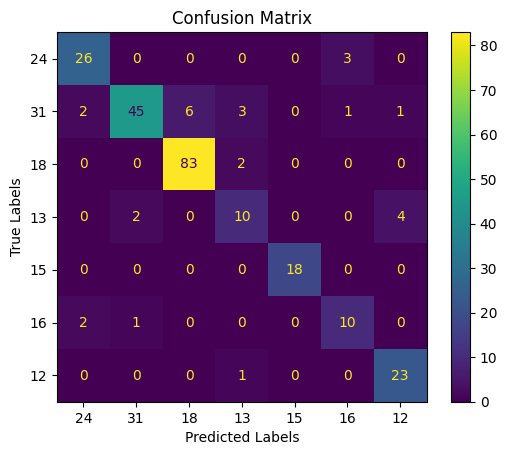
\includegraphics[height=6cm]{report/figs/knn-confusion-matrix-first.png} }}
    \qquad
    \subfloat[\centering 14 food groups]{{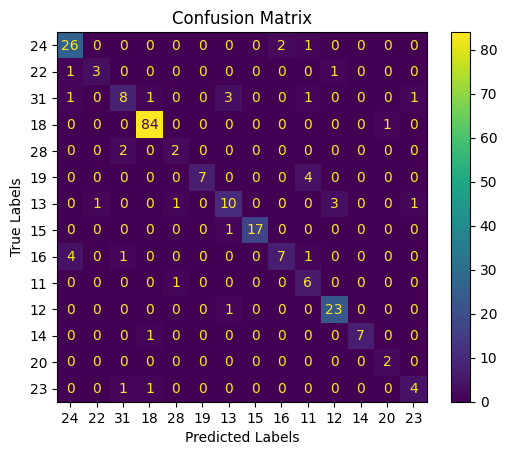
\includegraphics[height=6cm]{report/figs/knn-confusion-matrix-second.png} }}
    \qquad
    \subfloat[\centering 23 food groups]{{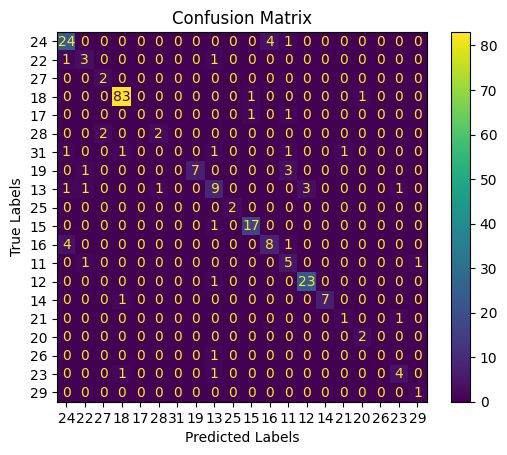
\includegraphics[height=6cm]{report/figs/knn-confusion-matrix-third.png} }}
    \caption{The confusion matrices for the \protect\UseVerb{topx} food group models.}
    \label{fig:confusion-matrices}
\end{figure}

In general, $k$-nn appears to perform better when classifying a smaller number of food groups. In Table \ref{tab:table}, we can see that the $k$-nn performed best when classifying the top 6 food groups, beating all other variations in all accuracy metrics. We believe this is due to the fact that the model is able to more easily distinguish between the larger, more general food groups, due to the larger number of data points available for the those groups, as was seen in the distribution bar graph (Figure \ref{fig:food-group-distribution}). The confusion matrices (Figure \ref{fig:confusion-matrices}) here further validate this hypothesis, as we can see the diagonal values get dimmer and dimmer as the number of food groups increases.

\section{Discussion}
\emph{Why are your results significant and valuable?}

In this study, one specific aspect of the pre-processing was of particular interest: the number of food groups to be collated by the miscellaneous group. Three different variations of the data were created, focusing on the top 6, 14 and 23 largest food groups. All variations of our model were well above a conservative 75\% accurate, which is an indication that the model is effective and somewhat reliable.
Across the board, as the number of food groups increased, the accuracy of predicting the specific food group for each item decreased; the knn model with 6 groups performed better than the models with 14 and 23 groups, respectively. This indicates that the model performs better in categorising foods into larger, more general food groups, but struggles with smaller, more nuanced groups. This could be due to multiple reasons, such as: the model struggling to recognise trends and patterns in groups of very little data, and these smaller groups being inherently more complex in nature. Less populated food groups are likely to be areas of ambiguity; the foods may be uncommon or even delicacies, such as in the case of group 34, ‘Reptiles, amphibia and insects’. These foods are also not necessarily categorised by their nutritional value, but rather their origin or specific purpose, such as group 30, ‘Special dietary foods’. Where these labels are determined on factors other than nutritional values, the model begins to encounter difficulties.
This highlights a limitation of the dataset, and thus suggests there are restraints to the supervised learning model’s accuracy. This analysis also supports the notion that pre-processing techniques also significantly influence the data and the resultant predictions, emphasising the importance of careful consideration and understanding of the potential effects of pre-processing methods. Additionally, the very consistent improvement of the model where food groups are simplified strongly suggests that if this process were to be conducted again, the model could become even more effective and accurate with a more balanced and rich dataset.

\subsection{Evaluation Methods}
To ensure that a single evaluation method did not inspire overconfidence in the results of this data, we employed cross validation and bootstrap validation, to generate accuracy scores and graphs, and confusion matrices. The predictive model we constructed was found to be generally highly accurate in determining food groups from nutritional values, exhibiting an 70 - 90\% accuracy range across the three different methods of accuracy verification.
In the bootstrap validation, the high precision of 75 - 88\% ensures reliable positive predictions while the high recall of 70 - 90\% infers accurate identification of data. The high F1 score indicates that the model is successful in achieving both high precision and high recall, making it a reliable tool predicting food groups based on nutritional information.



The cross validation of the knn models produced accuracy scores ranging from ~79 to 87\%. This illustrates that the model still has compelling effectivity even when trained and tested on a variety of different partitioning of the data into train and test sets. This means that the model has good generalisability and predictive capability. However, these cross-validation scores being lower than the initial model does suggest that the initial implementation of the knn model was perhaps endowed with a test set primarily consisting of strongly identifiable food groups.

There also exists the potential issue of overfitting within and thus overconfidence inspired by the bootstrap validation. The bootstrap validation scores are generally higher than the cross-validation scores, suggesting that the model is performing better on resampled data compared to the original data. The difference is not so large that this is of major concern, however this is some reason to cautiously question and doubt the upper bounds of the apparent accuracy of this model. 

However, these high accuracy rates still allow margins for error, which could be problematic in a practical application of this model. For example, considering the vast number of food items found in a supermarket, an error rate of approximately 15\%, as our data suggests, would still require a great deal of manual data checking which would be time-consuming and challenging. Considering if the model did not 100\% accurately label groups, it may provide a bad shopping experience for supermarket chains’ customers, with foods being in the wrong places, or perhaps even endangering customers, who may be placed in danger due to perhaps, anaphylaxis or other dietary health concerns. Thus, there may be a need for a significant amount of manual checking, which can be costly in terms of time and labour. In its current state, trained only on the data we were provided in this project, this model may not be suitable for immediate implementation and reliance on in this specific use case. 




\section{Conclusion}
\emph{What are the limitations of your results and how can the project be improved for future?}

Throughout this investigation, we gained valuable insights into the data processing pipeline. The processes and strategies we utilised in preprocessing and analysis of the data elucidate the relationship between nutritional values and food groupings. With the ultimate goal of exploring and answering the question of ‘to what extent can we predict the food group of a food item based solely on its nutritional information?’,  this research endeavour has demonstrated this is entirely possible to achieve. It has also shown that the effectiveness of this enterprise is dependent on not only the initial data available, but also highly contingent on early-stages data cleaning and preparation. The validation and evaluation we conducted on our KNN models supportively indicate that this is generally a successful way of predicting food groups, despite the aforementioned limitations. Future investigations of similar nature would tremendously benefit from use of a more well-rounded and balanced data set, given that some classifications in this data set have as few as one or two food items. With a much larger dataset, future experiments could also aim to classify sub-groups, i.e., minor food groups, rather than major.


\newpage
\bibliographystyle{plainnat}
\bibliography{references}


\end{document}
